\documentclass[preprint,11pt]{elsarticle}
\usepackage{geometry}               
\geometry{letterpaper}                  
\usepackage{graphicx}
\usepackage{amssymb,amsmath}
\usepackage{epsfig,subfigure,epstopdf}
\usepackage{algorithm}
\usepackage{algorithmic}
\usepackage{rotating}

% -- David Package --
\usepackage[normalem]{ulem}
\usepackage[usenames,dvipsnames]{color}
\newcommand{\rd}{\textcolor{Red}}
\newcommand{\gr}{\textcolor{Green}}
\newcommand{\og}{\textcolor{Orange}}
\newcommand{\pp}{\textcolor{Purple}}
\usepackage[edtable]{lineno}
% -- End of package --

\newtheorem{theorem}{Theorem}[section]
\newtheorem{lemma}[theorem]{Lemma}
\newtheorem{proposition}[theorem]{Proposition}
\newtheorem{corollary}[theorem]{Corollary}
\newenvironment{proof}[1][Proof]{\begin{trivlist}
\item[\hskip \labelsep {\bfseries #1}]}{\end{trivlist}}
\newenvironment{definition}[1][Definition]{\begin{trivlist}
\item[\hskip \labelsep {\bfseries #1}]}{\end{trivlist}}
\newenvironment{example}[1][Example]{\begin{trivlist}
\item[\hskip \labelsep {\bfseries #1}]}{\end{trivlist}}
\newenvironment{remark}[1][Remark]{\begin{trivlist}
\item[\hskip \labelsep {\bfseries #1}]}{\end{trivlist}}

\DeclareGraphicsRule{.tif}{png}{.png}{`convert #1 `dirname #1`/`basename #1 .tif`.png}

\begin{document}
\begin{frontmatter}
  \title{General Linear Algebra Computing Environment}
  \author[a01]{Chenhan D. Yu} \ead{chenhan@cs.utexas.com}
  \author[a01]{Jianyu Huang} \ead{jianyu@cs.utexas.com}
  \address[a01]{Department of Computer Science, University of Texas at Austin}

  \begin{abstract}
  GLACE is a runtime system freeing user from writing multiple parallel APIs, 
  learning parallel algorithms, yet at the same time still fully exploit the computing power 
  of heterogeneous systems.
   
  After the Moore law broke, architectures of modern computers become much more 
  complex than before. The performance of sequential code is no longer portable and 
  scalable on new architectures, and the burden again goes back to programmers. 
  Recently, in order to deploy all computing resources, programmers may need to learn 
  OpenMp or Pthread for shared memory systems, MPI or socket programming for 
  distributed systems, CUDA, OpenCL or OpenGL if the system is equipped with 
  accelerators.
  
  Of course, learning these languages doesn't solve the problem. Even if programmers can 
  write these languages, they are still far away from getting high performance, since these 
  languages are just virtual programming models that facilitate programming, yet the actual 
  behaviors mapping to the hardware are hidden. An automatic parallelizing environment is 
  needed to avoid these inefficient developing processes.
  
  So our goal is to provide programmers with such an automatic parallelizing environment 
  in the domain of linear algebra. By dependency analysis, we are able to transform this 
  problem into a scheduling problem which will be solved by some new heuristic algorithms 
  later. The dependency analysis is implemented on domain languages level (a.k.a task 
  level) but not instruction level to take the advantage of some existing high performance 
  libraries such as BLAS, LAPACK.
  
  Note that the just in time (JIT) analysis frees users from any control flow, loop or function 
  call issue in parallel computing, but still cheap enough, since tasks are much fewer than 
  instructions. We compare the similarity between the existing static instruction scheduling 
  strategies and our dynamic strategies, contrasting the difference to show the limitation of 
  static analysis. At the end we will also show how this environment and the just in time 
  analysis is useful by both dense and sparse matrix computation.
  \end{abstract}
  \begin{keyword}
    Automatic parallelism \sep Task scheduling \sep
    heterogenous computing \sep graphic processing unit (GPU) \sep Intel Xeon Phi
  \end{keyword}
\end{frontmatter}

\linenumbers \linenumberdisplaymath

% ====================================================================
\section{Introduction}
% ====================================================================
  After the Moore law broke, architectures of modern computers become much more 
  complex than before, and the performance of sequential code is no longer portable and 
  scalable on new architectures. The burden again shifts from system designers back to 
  programmers, since automatic parallelization in the compiler level is still a difficult problem to 
  solve. Thus, most of the programmers choose to control multiple threads or processes 
  themselves in order to exploit the computing resources.  
  
  Recently, in order to deploy all computing resources, programmers may need to learn 
  OpenMp \cite{} or Pthread \cite{} for shared memory systems, MPI \cite{} or socket 
  programming for distributed systems, CUDA \cite{}, OpenCL \cite{} or OpenGL \cite{} if the 
  system is equipped with accelerators. 
  All the APIs above require programmers to control threads or processes explicitly, and
  OpenMP is the only API with compiler support automatic parallelization that allow user to 
  use annotations to specify the parallel section. Unfortunately, this kind of parallel model (BSP)
  has a critical problem in synchronization for unbalance loading and also is not suitable for
  heterogenous system.   
  
  
% ====================================================================
\section{Dependency Analysis}
% ====================================================================
  GLACE allows users to write their program in a sequential fashion and performs run-time
  dependency analysis to exploit parallelism. Top level routines will be partitioned into smaller
  tasks that can have 3 different kinds of dependency: write after read (WAR), read after
  write (RAW), write after write (WAW). Two tasks with one of these dependencies can't 
  be executed concurrently otherwise may lead to incorrect results. 
  In GLACE, the analysis phase will be performed after the task generating by 
  using Algorithm ~\ref{alg:dep}. The algorithm is a simplified version of the dependency 
  analysis in \cite{}.     


  %Especially for the submatrix part...


  dependecy analysis


  Ernie Chan


  True(Flow) dependency
  Flow dependencies occur where a block is read by one task after it is written by a previous task (read after write).
  e.g.
  S1: A := B + C;


  Anti-dependency
  Anti-dependencies creates the scenarios when one task write a block after another task read the same task. (write after read).
  e.g.

  Output dependency
  Output dependency 


  focus

  flow dependency notation


  The figure is too ugly. I think we may need to add the subscript to the symbol so that it looks a little "acceptable".

  Instruction Scheduling


  Difference with Ernie Chan's work.




  Constructing a DAG
 



% ====================================================================
\section{Data Distribution and Software Cache}
% ====================================================================
  In order to increase the data reuse rate and reduce the overhead of communication, GLACE
  implements a software cache to manage device memory. We use IMP model \cite{} to 
  describe an distribution of an object's location. This enable GLACE to analysis data affinity
  between tasks easily and also reduce the overhead of cache table looking up.
  
  Although GLACE is targeting on shared memory system, yet we treat the device memory
  as a kind of distributed memory. An object's distribution can only have one copy in the 
  host memory or on the certain device, or can have several copies across the host and
  devices. For example, if the system has 4 devices, there $(4+1)^2 - 1$ possible distributions.
  Here, we further assume that each device has no connection between each other. Thus,
  there are only $4 + 4^2$ possible distributions, since it's impossible that 2 devices have 
  the object, but it isn't in the host memory. 
    
% ====================================================================
\section{Heterogenous Performance Model}
% ====================================================================
  GLACE try to solve the optima heterogenous schedule problem by assuming that there is 
  a performance model for each task on each architecture. The performance model includes
  computation cost and communication cost. By using this model, GLACE is able to balance
  the workload on each worker and also reduces the communication amount.  

% ====== < Notation Table > ======
\begin{table}
  \centering
  {\footnotesize 
  \begin{tabular}{lllll}
    \hline
    Notation    &\ & Meaning of the notation \\  \cline{1-1}  \cline{3-3}
    {\tt nw}        && number of workers \\
    {\tt nt}          && number of tasks \\
    {\tt k}           && number of supernodes \\
    {\tt sn$_i$}  && row dimension of $F_1$ in the $i$th frontal \\
                       && (also the number of pivoting column in a supernode) \\
    {\tt up$_i$}  && row dimension of $F_2$ in the $i$th frontal \\
                       && (also the number of non-pivoting column in a supernode) \\ 
    \hline
    $SF^c$  && CPU time for symbolic factorization and elimination tree construction.\\
    $CH^c(s)$ or $CH^g(s)$     && CPU or GPU time for Cholesky factorization $F_1=L_1L_1^{T}$ \\
    $TR^c(s,u)$ or $TR^g(s,u)$ && CPU or GPU time for triangular solves $L_2 = F_2L_1^{-T}$\\
    $SC^c(s, u)$ or $SC^g(s, u)$     && CPU or GPU time for updating Schur complement $U = C - L_2L_2^{T}$ \\
    $BL^c(s,u)$ or $BL^g(s,u)$ && BLAS3 costs on CPU or GPU that\\
    && $BL^c(s,u) = CH^c(s) + TR^c(s, u) +SC^c(s, u)$ and\\
    && $BL^g(s,u) = CH^g(s) + TR^g(s, u) +SC^g(s, u)$\\\hline

    $AD^c(s, u)$ or $AD^g(s, u)$   && CPU or GPU time for assembling (add elements) of a {\tt s}$\times${\tt (s+u)} matrix \\
    $AS^c(u)$ or $AS^g(u)$   && CPU or GPU time for assembling of a {\tt u}$\times${\tt u} matrix \\ \hline

    $CP^c_i$ or $CP^g_i$ && Computation cost of {\tt i}th frontal on CPU or GPU\\
    $CP^c$ or $CP^g$ && Overall computation cost on CPU or GPU\\ \hline

    $CM^c$ or $CM^{g}$ && Overall communication cost  on CPU or GPU\\
    $ \widehat{CM}^{g}$ && Overall communication cost  on GPU by using asynchronized memory copy. \\
    $CM^A$ or $CM^{ET}$ && Communication cost of the coefficient matrix $A$ or
the elimination tree\\

    {\tt $V_{cg}$} && Communication efficiency (bytes/sec) between CPU and GPU \\ \hline

    ${\tt gpu_i}$ && indicator for the $i$th frontal is perform on GPU
(${\tt gpu_i}=1$) or CPU (${\tt gpu_i}=0$)\\
    ${\tt cpu_i}$ && indicator for the $i$th frontal is perform on GPU or CPU (${\tt cpu_i}=1-{\tt gpu_i}$)\\
    ${\tt p_i}$ && the parent frontal of $i$th frontal\\
    ${\tt gpu_{p_i}}$ &&  the parent of the {\tt i}th frontal is factored on GPU or not (${\tt gpu_{p_i}}=$ 1 or 0)\\
    \hline
  \end{tabular}
}
\caption{Notations used in the hybrid CPU-GPU multifrontal methods.
  The variable $s$ and $u$ stand for the dimension of the matrix corresponding 
  to {\tt sn$_i$} and {\tt up$_i$}.}
  \label{tab:notation}
\end{table}
% ------  

% ====================================================================
\section{Scheduler}
% ====================================================================
  GLACE scheduler is responsible for queuing ready tasks to workers' ready queue. 

\begin{figure}
  \centering
  \includegraphics[width=6.0in]{output1.eps} 
  \caption{1-by-1 partition}
  \label{fig:dep1}
\end{figure}
\begin{figure}
  \centering
  \includegraphics[width=6.0in]{output.eps} 
  \caption{2-by-2 partition}
  \label{fig:dep2}
\end{figure}

\begin{figure}
\begin{minipage} [t] {0.5\textwidth}
  \includegraphics[width=3.2in]{timeline1.eps} 
  \caption{Execution timeline without prefetching, green(communication), red(computation)}
  \label{fig:timeline1}
\end{minipage}
\begin{minipage} [t] {0.5\textwidth}
  \includegraphics[width=3.2in]{timeline2.eps} 
  \caption{Execution timeline without prefetching, green(communication), red(computation)}
  \label{fig:timeline2}
\end{minipage}
\end{figure}

\begin{algorithm}
\caption{{\bf (estimate).} GLACE cost estimation algorithm}
\label{alg:estimate}
{\footnotesize
\begin{algorithmic} [1]
\STATE C = estimate(worker, task)
\STATE Input: worker, task
\STATE Output: C
\STATE $CM = 0$, $CP = 0$
\IF {worker.device}
  \STATE $CP = model(worker.device, task, arguments)$
  \FOR {each argument of the task}
    \IF {worker.device $\notin$ distribution}
      \STATE $CM \pm bandwidth(sizeof(argument))$
      \IF {host $\notin$ distribution}
        \STATE $CM \pm bandwidth(sizeof(argument))$
      \ENDIF
    \ENDIF
  \ENDFOR 
\ELSE
  \STATE $CP = model(host, task, arguments)$
  \FOR {each argument of the task}
    \IF {host $\notin$ distribution}
      \STATE $CM \pm bandwidth(sizeof(argument))$
    \ENDIF
  \ENDFOR 
\ENDIF
\STATE $C = CM + CP$
\end{algorithmic}
}
\end{algorithm}

\begin{algorithm}
\caption{{\bf (fetch).} GLACE fetch algorithm}
\label{alg:fetch}
{\footnotesize
\begin{algorithmic} [1]
\STATE fetch(worker, task)
\STATE Input: worker, task
\FOR {each argument of the task}
  \STATE acquire the distribution lock   
  \IF {worker.device $\notin$ distribution}
    \IF {host $\notin$ distribution}
      \STATE pick a source from the distribution and $cache\_writeback()$
      \STATE distribution $=$ distribution $\cup$ host
    \ENDIF
    \IF {worker.device}
      \STATE $cache\_fetch()$
      \STATE distribution $=$ distribution $\cup$ worker.device
    \ENDIF
  \ENDIF
  \STATE acquire the lock of device cache
  \STATE release the distribution lock
\ENDFOR
\end{algorithmic}
}
\end{algorithm}

\begin{algorithm}
\caption{{\bf (prefetch).} GLACE prefetch algorithm}
\label{alg:prefetch}
{\footnotesize
\begin{minipage} [t] {0.4\textwidth}
\begin{algorithmic} [1]
\STATE $d2h = prefetch\_d2h(worker)$
\STATE Input: worker
\STATE Output: d2h
\IF {! isempty(worker.writeback)}
  \STATE object = head(worker.writeback)
  \IF {host $\notin$ distribution}
    \STATE $cache\_async\_writeback()$
    \STATE return TRUE
  \ENDIF
\ENDIF
\STATE return FALSE
\end{algorithmic}
\end{minipage}
\begin{minipage} [t] {0.6\textwidth}
\begin{algorithmic} [1]
\STATE $h2d = prefetch\_d2h(worker)$
\STATE Input: worker
\STATE Output: h2d 
\IF {! isempty(worker.readyqueue)}
  \STATE task $=$ head(worker.readyqueue)
  \FOR {each argument of the task}
    \IF {worker.device $\notin$ distribution}
      \IF {host $\in$ distribution}
        \STATE $cache\_async\_fetch()$
        \STATE acquire the distribution lock
        \STATE distribution $=$ distribution $\cup$ worker.device
        \STATE release the distribution lock
      \ENDIF
    \ENDIF
  \ENDFOR
\ENDIF
\end{algorithmic}
\end{minipage}
}
\end{algorithm}

\begin{algorithm}
\caption{{\bf (execute).} GLACE execute algorithm}
\label{alg:execute}
{\footnotesize
\begin{algorithmic} [1]
\STATE $execute(worker, task)$
\STATE Input: worker, task
\STATE $fetch(worker, task)$
\STATE d2h $=$ $prefetch\_d2h(worker)$
\STATE h2d $=$ $prefetch\_h2d(worker)$
\STATE $kernel(arguments)$
\FOR {each W or RW type argument of the task}
  \STATE distribution $=$ worker.device
  \STATE $push\_tail(worker.writeback)$  
\ENDFOR
\STATE $wait\_prefetch(worker, d2h, h2d)$
\end{algorithmic}
}
\end{algorithm}

\begin{algorithm}
\caption{{\bf (update).} GLACE dependencies update algorithm}
\label{alg:update}
{\footnotesize
\begin{algorithmic} [1]
\STATE $update(task)$
\STATE Input: task
\STATE
\end{algorithmic}
}
\end{algorithm}


\begin{algorithm}
\caption{{\bf (update).} GLACE dependencies analysis algorithm}
\label{alg:update}
{\footnotesize
\begin{algorithmic} [1]
\STATE $update(task)$
\STATE Input: Linear algebra algorithm S, block size b
\STATE Output: Directed acyclic graph (V, E)
\STATE V :=  empty set; E := empty set;
for each matrix A \in R^{m \times n}
  for i from 0 to m/b do
    for j from 0 to n/b do
	  A(i,j) -> reset = empty set; A(i,j) -> wset = empty set;
	end for
  end for
end for

A_ij   represents the ith in row, jth in column submatrix???? blocks
for each \textbf{task} in S
Store task into the Vertex Set: V: = V \union {task}
for each A(i,j) read / rw by task do
A(i,j)->rset :=  A(i,j)->rset \union {task}
if (A(i,j)->wset != empty_set) 
  for each element t' in A(i,j)->wset 
  	if task != t' then 
		add edge E:= E \union {t' -> t}
	end if
  end for
end if
end for


for each A(i,j) write / rw by task do
if (A(i,j)->rset != empty_set)
  for each element t' in A(i,j)->rset
    if task != t' then
		add edge E:= E \union {t' -> t}
	end if
  end for
end if
end for


%Submatrix -> 


\end{algorithmic}
}
\end{algorithm}






\begin{algorithm}
\caption{{\bf (worker).} GLACE worker algorithm}
\label{alg:worker}
{\footnotesize
\begin{algorithmic} [1]
\STATE $worker(worker)$
\STATE Input: worker
\WHILE {! isempty(worker.readyqueue)}
  \STATE acquire the readyqueue lock
  \STATE task $=$ $pop\_head(worker.readyqueue)$
  \STATE release the readyqueue lock
  \IF {task}
    \STATE commit $=$ $execute(worker, task)$;
    \IF {commit}
      \STATE update dependencies
    \ENDIF
  \ENDIF
\ENDWHILE
\end{algorithmic}
}
\end{algorithm}

%----------------------------------------------------------------------------------------

\end{document}
